% Emerald Publishing - Construction Innovation Submission Template
% by Oleksandr Melnyk
% Ver 0.0.4
% Based on: https://www.emeraldgrouppublishing.com/journal/ci#author-guidelines


\documentclass{article}

\usepackage[english]{babel}

% Set page size and margins
% Replace `letterpaper' with `a4paper' for UK/EU standard size
\usepackage[a4paper,top=2cm,bottom=2cm,left=3cm,right=3cm,marginparwidth=1.75cm]{geometry}

% Useful packages
\usepackage{amssymb}
\usepackage{siunitx}
\PassOptionsToPackage{hyphens}{url}\usepackage{hyperref}
\usepackage{cleveref}
\usepackage[utf8]{inputenc}
\usepackage[right]{lineno}
\usepackage{csquotes}
\usepackage{booktabs}
\usepackage{longtable}
\usepackage{adjustbox}
\usepackage{array}
\usepackage{url}
\usepackage{titlesec}
%\usepackage[compatibility=false]{caption}
\usepackage{authblk}
\usepackage{xcolor} % Load the xcolor package for color options
\renewcommand{\thetable}{\Roman{table}}

% Define a new format for \subsection
\titleformat{\subsection}
  {\mdseries\itshape\large} % Medium series, italic shape, and large font size
  {\thesubsection}{1em}{} % Numbering, spacing, and the section title itself


% Emerald Harvard Citation Style

\usepackage[english]{babel}
\usepackage[style=authoryear,backend=biber,natbib=true,maxcitenames=2,uniquelist=false]{biblatex}
\addbibresource{bibliography.bib} % your .bib file

% Customizing biblatex for Harvard style
% Customizing biblatex for Harvard style
\DeclareNameAlias{sortname}{family-given}
\DeclareNameAlias{default}{family-given}

\renewbibmacro{in:}{}
\DeclareFieldFormat[article]{title}{\mkbibquote{#1}\addcomma}
\DeclareFieldFormat[book]{title}{\mkbibemph{#1}\addcomma}
\DeclareFieldFormat[bookinbook]{title}{\mkbibemph{#1}\addcomma}
\DeclareFieldFormat[inbook]{title}{\mkbibquote{#1}\addcomma}
\DeclareFieldFormat[incollection]{title}{\mkbibquote{#1}\addcomma}
\DeclareFieldFormat[inproceedings]{title}{\mkbibquote{#1}\addcomma}
\DeclareFieldFormat[manual]{title}{\mkbibemph{#1}\addcomma}
\DeclareFieldFormat[misc]{title}{\mkbibemph{#1}\addcomma}
\DeclareFieldFormat[thesis]{title}{\mkbibemph{#1}\addcomma}
\DeclareFieldFormat[unpublished]{title}{\mkbibquote{#1}\addcomma}
\DeclareFieldFormat[patent]{title}{\mkbibemph{#1}\addcomma}
\DeclareFieldFormat[report]{title}{\mkbibemph{#1}\addcomma}
\DeclareFieldFormat[online]{title}{\mkbibquote{#1}\addcomma}
\DeclareFieldFormat[software]{title}{\mkbibemph{#1}\addcomma}
\DeclareFieldFormat[booklet]{title}{\mkbibemph{#1}\addcomma}
\DeclareFieldFormat[periodical]{title}{\mkbibemph{#1}\addcomma}
\DeclareFieldFormat[standard]{title}{\mkbibemph{#1}\addcomma}

\DeclareFieldFormat[article]{journaltitle}{\iffieldundef{shortjournal}{\mkbibemph{#1}\addcomma}{\mkbibemph{\printfield{shortjournal}}\addcomma}}
\DeclareFieldFormat{volume}{\bibstring{volume}~#1}
\DeclareFieldFormat{number}{\bibstring{number}~#1}

% Definitions for "Vol." and "No."
\DefineBibliographyStrings{english}{
  volume = {Vol.},
  number = {No.}
}

\renewbibmacro*{volume+number+eid}{%
  \printfield{volume}%
  \setunit*{\addspace}%
  \printfield{number}%
  \setunit{\addcomma\space}%
  \printfield{eid}}

\renewbibmacro*{journal+issuetitle}{%
  \usebibmacro{journal}%
  \setunit*{\addcomma\space}%
  \usebibmacro{volume+number+eid}%
  \setunit{\addcomma\space}%
  \usebibmacro{issue+date}}

\renewbibmacro*{publisher+location+date}{%
  \printlist{publisher}%
  \iflistundef{location}
    {\setunit*{\addcomma\space}}
    {\setunit*{\addcolon\space}}%
  \printlist{location}%
  \setunit*{\addcomma\space}%
  \usebibmacro{date}}

\renewcommand*{\bibpagespunct}{\addcomma\space}

% Customizing page field format to prevent duplication
% \DeclareFieldFormat{pages}{%
%   \mkfirstpage[{\mkpageprefix[page]{#1}}]{#1}}

% Customizing citations for Harvard style
\DeclareCiteCommand{\cite}[\mkbibparens]
  {\usebibmacro{prenote}}
  {\usebibmacro{citeindex}%
   \usebibmacro{cite}}
  {\multicitedelim}
  {\usebibmacro{postnote}}

\renewbibmacro*{cite:labelyear+extrayear}{%
  \iffieldundef{labelyear}
    {}
    {\printtext[bibhyperref]{%
       \printfield{labelyear}%
       \printfield{extrayear}}}}

\renewbibmacro*{cite:labeldate+extradate}{%
  \iffieldundef{labelyear}
    {}
    {\printtext[bibhyperref]{%
       \printfield{labelyear}%
       \printfield{extradate}}}}

\AtEveryBibitem{
  \clearfield{month}
  \clearfield{day}
  \ifentrytype{book}{
    \clearlist{location}
  }{}
}

% Formatting "et al." in italics followed by a comma
\DefineBibliographyStrings{english}{
  andothers = {\textit{et al.},}
}

\DeclareFieldFormat[article]{volume}{\bibstring{jourvol}\addnbspace #1}
\DeclareFieldFormat[article]{number}{\bibstring{number}\addnbspace #1}
\DeclareFieldFormat[article]{volume}{Vol. #1}
\DeclareFieldFormat[article]{number}{No. #1}
% Customizing DOI field format to lowercase "doi"
%\DeclareFieldFormat{doi}{\bibstring{doi}\addcolon\space\url{#1}}

% Customizing URL field format to "available at:"
\DeclareFieldFormat{url}{\bibstring{available at}\addcolon\space\url{#1}}
\DeclareFieldFormat{urldate}{\mkbibparens{accessed \addspace#1}}

% Customizing urldate to match the required format
\DeclareFieldFormat{urldate}{%
  \mkbibparens{accessed\space%
    \thefield{urlday}\addspace%
    \mkbibmonth{\thefield{urlmonth}}\addspace%
    \thefield{urlyear}}}

% Configure cleveref
\crefformat{figure}{#2Figure~#1#3}
\Crefformat{figure}{#2Figure~#1#3}
\crefformat{table}{#2Table~#1#3}
\Crefformat{table}{#2Table~#1#3}
\crefformat{section}{#2Section~#1#3}
\Crefformat{section}{#2Section~#1#3}

%Front Matter
\author[1]{Colli Simone}
\author[2]{Merenda Saverio Mattia}

\affil[1]{
    \url{simone.colli@studenti.unipr.it}
    }
\affil[2]{
    \url{saveriomattia.merenda@studenti.unipr.it}
    }

% Titolo
\title{Titolo da mettere}

\begin{document}
\maketitle
\begin{abstract}
    Questo lavoro presenta l'analisi e l'implementazione di un sistema automatizzato per 
    l'assegnazione dei garanti ai corsi universitari, in conformità ai requisiti ministeriali. 
    L'obiettivo principale è garantire che ogni corso soddisfi i vincoli minimi di docenza, 
    rispettando le regole di distribuzione tra diverse categorie di docenti e ottimizzando 
    l'uso delle risorse disponibili.

    Utilizzando la programmazione logica con Answer Set Programming (ASP), 
    abbiamo modellato il problema attraverso fatti, regole e vincoli derivati dai dati 
    ministeriali e universitari. Abbiamo implementato una serie di vincoli per rispettare 
    i minimi richiesti di docenti per corso, evitando sovrapposizioni improprie tra gli 
    incarichi dei docenti e considerando scenari realistici in cui un docente può assumere 
    più ruoli parziali.
    
    L'approccio è stato testato su un dataset reale contenente informazioni su corsi, SSD 
    (Settori Scientifico Disciplinari) e docenti dell'Università degli Studi di Parma. 
    I risultati dimostrano come il sistema possa trovare configurazioni ottimali che 
    soddisfano i requisiti, massimizzando l'efficienza e mantenendo flessibilità 
    nell'assegnazione dei docenti.

\end{abstract}
% \linenumbers % utilizzato per debug
\section{Introduzione}
\label{sec:introduction}

L'assegnazione dei garanti nei corsi universitari costituisce una 
questione fondamentale per la gestione ottimale delle risorse accademiche. 
Nell'ambito universitario, il \textit{garante} è un docente responsabile 
di rappresentare e tutelare la qualità didattica di un corso, garantendo 
il rispetto dei requisiti disciplinari e istituzionali. I garanti possono 
appartenere a diverse categorie contrattuali: docenti a tempo indeterminato, 
docenti a tempo determinato e, in casi eccezionali, docenti a contratto.

La sfida principale consiste nel soddisfare i vincoli ministeriali 
relativi ai garanti, garantendo al contempo un'allocazione equilibrata 
e sostenibile delle risorse. Ogni corso deve essere supportato da un 
numero minimo di garanti, suddivisi tra le diverse fasce contrattuali, 
per assicurare un livello adeguato di competenza e rappresentatività. 
Inoltre, è indispensabile che almeno il 50\% dei garanti afferisca al 
Settore Scientifico Disciplinare (SSD) caratterizzante del corso, al 
fine di garantire la coerenza tra l'offerta formativa e le competenze 
disciplinari.

Un'ulteriore complessità è rappresentata dall'impiego di docenti a 
contratto, il cui utilizzo deve essere limitato e subordinato alle 
sole situazioni in cui non sia possibile soddisfare i requisiti 
attraverso i docenti strutturati. La necessità di rispettare questi 
vincoli, combinata con la disponibilità limitata di personale e la 
necessità di bilanciare il carico di lavoro, rende questo problema 
una sfida organizzativa e computazionale significativa.

Un primo ostacolo affrontato in questo progetto riguarda la fase di 
pre-elaborazione dei dati forniti dall'università, descritta nella 
Sezione~\ref{sec:pre-proc} di questo elaborato. I dati risultano 
disomogenei e incompleti, richiedendo una significativa pulizia e 
riorganizzazione prima di poter essere utilizzati efficacemente nel 
modello ASP. Questa fase ha richiesto lo sviluppo di strumenti 
dedicati per uniformare e validare i dati.

La Sezione~\ref{sec:asp} esplora il cuore del nostro approccio, 
ovvero la costruzione del modello ASP. Qui abbiamo implementato 
regole logiche per soddisfare i vincoli ministeriali e massimizzare 
l'efficienza dell'assegnazione dei garanti, tenendo conto delle 
limitazioni sulle fasce contrattuali e sull'impiego dei docenti a contratto.

Successivamente, nella Sezione~\ref{sec:expval}, presentiamo 
i risultati ottenuti su un esempio ridotto, un test che ha permesso 
di validare il modello in un ambiente controllato e di analizzare la qualità 
delle soluzioni generate. Infine, la Sezione~\ref{sec:dataset-tutti-dipartimenti} descrive 
l'applicazione del modello su un dataset completo contenente tutti i corsi 
universitari, eseguendo un benchmark su larga scala per valutare la 
capacità del nostro approccio di risolvere problemi reali e complessi.
\section{Main Section}
\label{sec:main_section}
When submitting manuscripts using \LaTeX, a PDF file must also be included. 
Articles should be between 6,000 and 10,000 words, encompassing all text, tables, and figures. 
A concise and descriptive title must be included, and it is essential to list all contributing authors in the submission, along with their email addresses, names, and affiliations.

\subsection{Subsection 1}
Ensure headings are concise and clearly indicate the hierarchy. 
Use sparingly and identify with consecutive numbers in square brackets.
Submit figures (such as \cref{fig-1} electronically at the highest resolution. Number figures consecutively with clear captions.

\begin{figure}[ht]
 \centering
 \makebox[\textwidth][c]{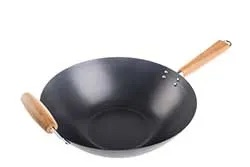
\includegraphics[width=1\textwidth]{images/padella.jpeg}}%
 \caption{Una padella}
 \label{fig-1}
\end{figure}

\subsection{Subsection 2}
\textbf{Emerald Publishing} accepts formats such as .ai, .eps, .jpeg, .bmp, and .tif. Electronic figures created in other applications should be provided in their original formats. 
Additionally, these figures should either be copied and pasted into a blank MS Word document or submitted as a PDF file.
\section{Conclusioni}
\label{sec:conclusion}


\hfill

\break
\printbibliography

\end{document}
